%% figures/fig3_small_model_regression.tex
%% Fig.3 — 모델 크기별 spec decode 효과 (회귀 → 이득 전환), 1컬럼

\begin{figure}[t]
\centering
\resizebox{0.95\columnwidth}{!}{%
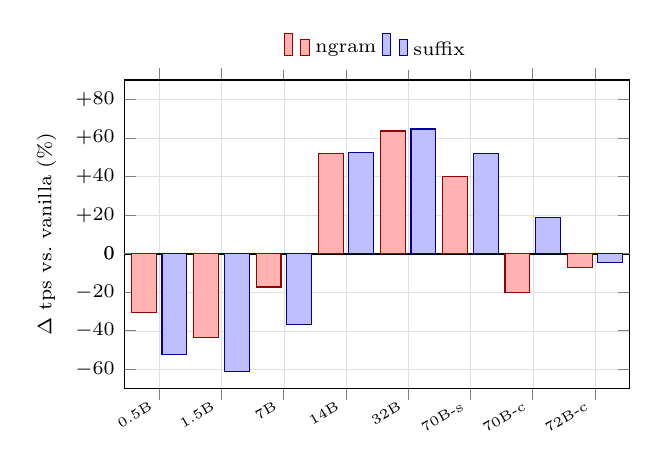
\begin{tikzpicture}
\begin{axis}[
    ybar=2pt,
    bar width=9pt,
    width=8cm, height=5.5cm,
    ylabel={$\Delta$ tps vs.\ vanilla (\%)},
    ylabel style={font=\scriptsize},
    symbolic x coords={0.5B, 1.5B, 7B, 14B, 32B, 70B-s, 70B-c, 72B-c},
    xtick=data,
    xticklabel style={font=\tiny, rotate=30, anchor=east},
    yticklabel style={font=\scriptsize},
    ymin=-70, ymax=90,
    ytick={-60,-40,-20,0,20,40,60,80},
    yticklabels={$-60$,$-40$,$-20$,$0$,$+20$,$+40$,$+60$,$+80$},
    legend style={at={(0.5,1.03)}, anchor=south, legend columns=2,
                  font=\scriptsize, draw=none},
    enlarge x limits=0.08,
    grid=major,
    grid style={line width=0.1pt, draw=gray!25},
    extra y ticks={0},
    extra y tick style={grid=major, grid style={black, thick}},
]
%% ngram (code workload baseline)
\addplot[fill=red!30, draw=red!60!black] coordinates {
    (0.5B,-30.5) (1.5B,-43.6) (7B,-17.3)
    (14B,52.0) (32B,63.6) (70B-s,40.1) (70B-c,-20.2) (72B-c,-7.4)};
%% suffix
\addplot[fill=blue!25, draw=blue!60!black] coordinates {
    (0.5B,-52.1) (1.5B,-60.9) (7B,-36.7)
    (14B,52.2) (32B,64.6) (70B-s,52.1) (70B-c,18.8) (72B-c,-4.6)};
\legend{ngram, suffix}
\end{axis}
\end{tikzpicture}%
}
\caption{모델 크기별 투기적 디코딩 효과.
  0.5B--7B 소형 모델은 ngram/suffix 모두 회귀(음수)를 보이고,
  14B 이상에서 양성으로 전환된다.
  단 Qwen-72B code는 suffix도 회귀($-4.6\%$).
  x축: model size / workload. 70B-s = sonnet, 70B-c = code, 72B-c = Qwen72B code.}
\label{fig:small-model-regression}
\end{figure}
